ابتدا توابع خروجی \lr{F} و \lr{G} را به‌دست می‌آوریم:

\begin{latin}
	\begin{itemize}
		\item 
		$ F=[A'\cdot (A'D)']' \cdot [BC + A'] = [A + (A'D)] \cdot [BC + A'] = ABC + A'BCD + A'D$
		
		\item 
		$ G=[A'D]' \cdot [A' + BC] = [A + D'] \cdot [A' + BC] = ABC + A'D' + BCD' $
	\end{itemize}
\end{latin}

سپس برای هر کدام از توابع \lr{F} و \lr{G} جدول کارنو رسم می‌کنیم.

برای تابع \lr{F} داریم:


\begin{latin}
	\begin{minipage}{0.48\textwidth}
		\centering
		\begin{karnaugh-map}[4][4][1][$B$][$A$][$D$][$C$](label=corner)
			\minterms{4,5,12,13,11,15}
			\implicant{4}{13}
			\implicant{15}{11}
		\end{karnaugh-map}
		\caption{K-Map 1}
		$$ (SOP):F=A'D + ABC $$
	\end{minipage}
	\hfill
	\begin{minipage}{0.48\textwidth}
		\centering
		\begin{karnaugh-map}[4][4][1][$B$][$A$][$D$][$C$](label=corner)
			\maxterms{0,1,2,3,6,7,8,9,10,14}
			\implicant{3}{6}
			\implicant{2}{10}
			\implicantedge{0}{1}{8}{9}
		\end{karnaugh-map}
		\caption{K-Map 2}
		$$ (POS):F=(A'+B) \cdot (C+A') \cdot (A+D) $$
	\end{minipage}	
\end{latin}




\begin{figure}[h]
	\centering
	\begin{subfigure}[b]{0.3\textwidth}
		\centering
		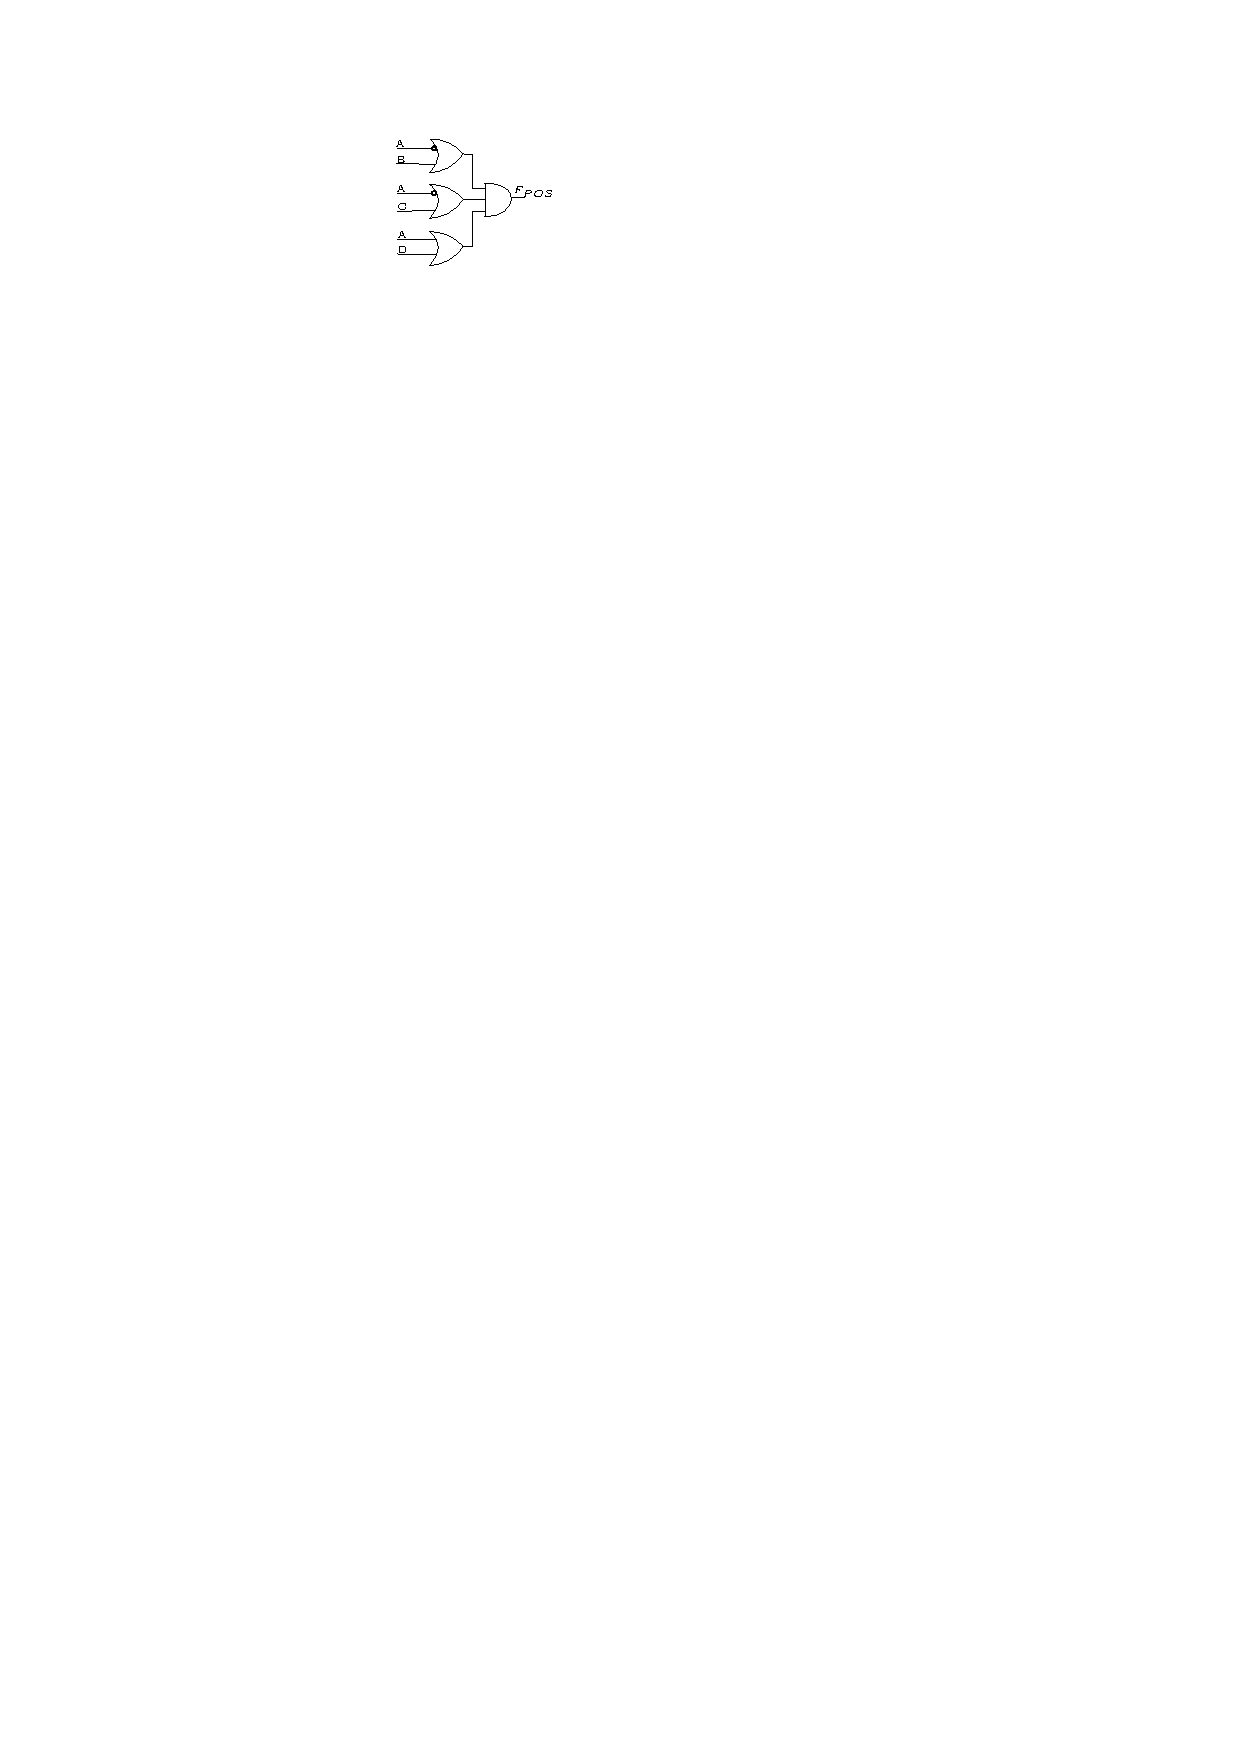
\includegraphics[width=\textwidth]{fig/Q1_F_POS.pdf}
		\caption{$F_{POS}$}
		\label{fig:F_POS}
	\end{subfigure}
	\hfil
	\begin{subfigure}[b]{0.3\textwidth}
		\centering
		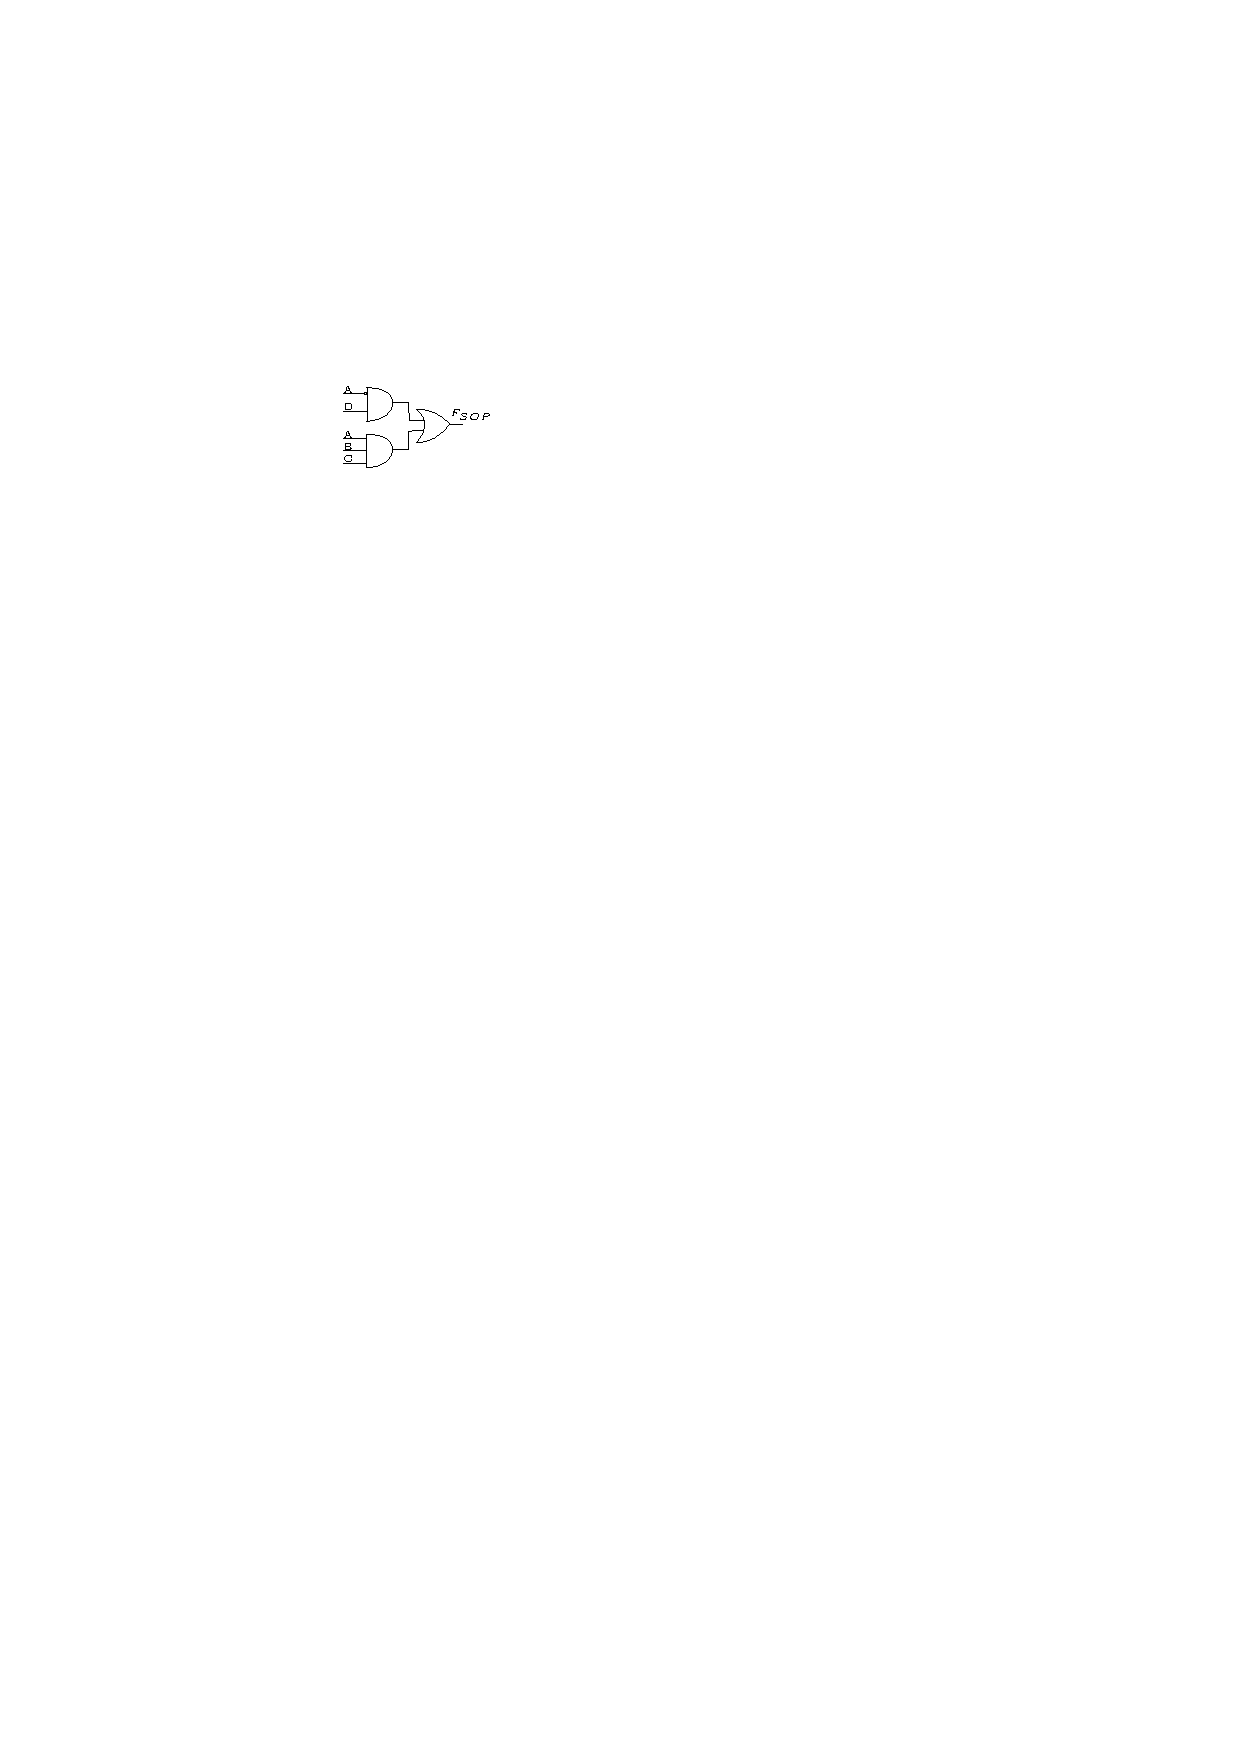
\includegraphics[width=\textwidth]{fig/Q1_F_SOP.pdf}
		\caption{$F_{SOP}$}
		\label{fig:F_SOP}
	\end{subfigure}
	\caption{مدار ساده شده تابع \lr{F}}
	\label{fig:مدار یاده شده اف}
\end{figure}




همچنین برای تابع \lr{G} داریم:


\begin{latin}
	\begin{minipage}{0.48\textwidth}
		\centering
		\begin{karnaugh-map}[4][4][1][$B$][$A$][$D$][$C$](label=corner)
			\minterms{0,1,8,9,11,15}
			\implicantedge{0}{1}{8}{9}
			\implicant{15}{11}
		\end{karnaugh-map}
		\caption{K-Map 1}
		$$ (SOP):G=A'D' + ABC$$
	\end{minipage}
	\hfill
	\begin{minipage}{0.48\textwidth}
		\centering
		\begin{karnaugh-map}[4][4][1][$B$][$A$][$D$][$C$](label=corner)
			\maxterms{2,3,4,5,6,7,10,12,13,14}
			\implicant{3}{6}
			\implicant{4}{13}
			\implicant{2}{10}
		\end{karnaugh-map}
		\caption{K-Map 2}
		$$ (POS):G=(A+D') \cdot (A'+C) \cdot (A'+B) $$
	\end{minipage}	
\end{latin}




\begin{figure}[h]
	\centering
	\begin{subfigure}[b]{0.3\textwidth}
		\centering
		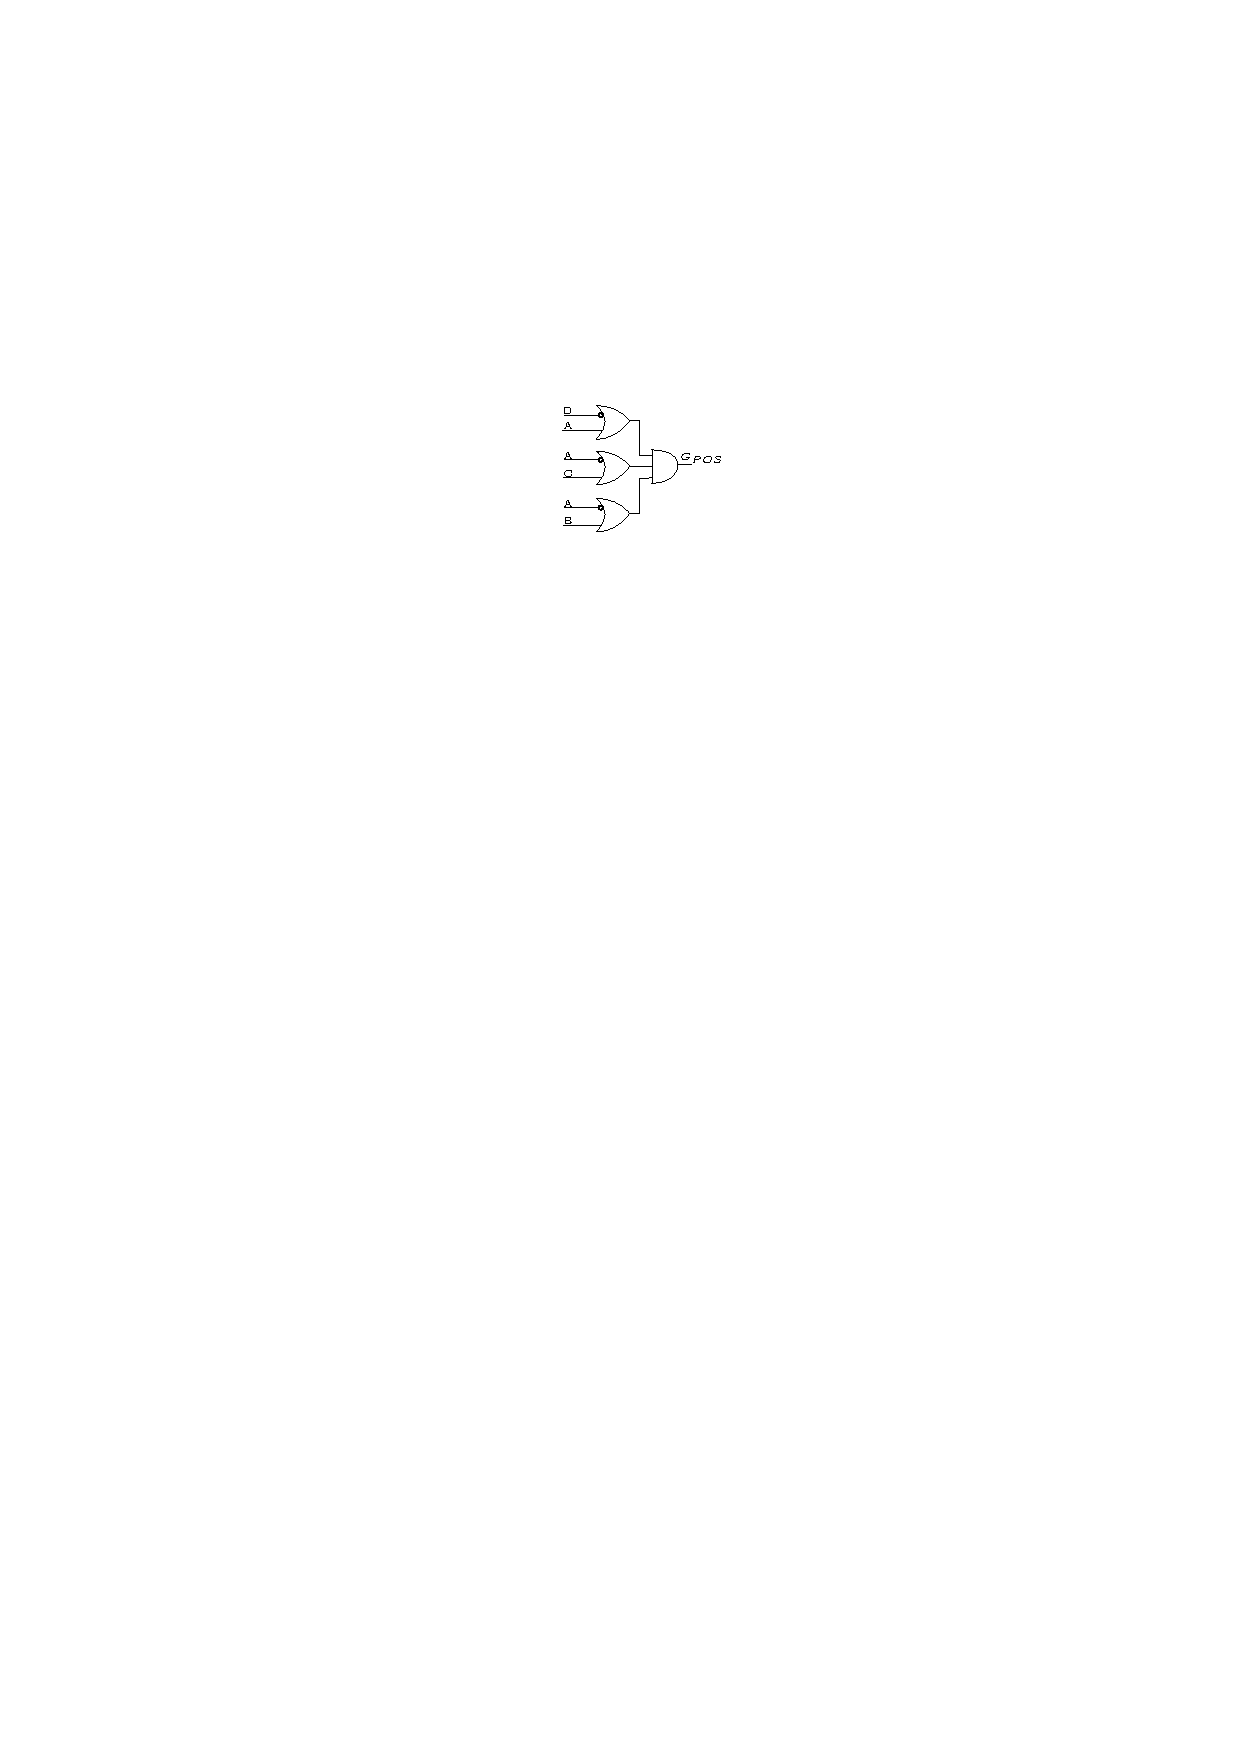
\includegraphics[width=\textwidth]{fig/Q1_G_POS.pdf}
		\caption{$G_{POS}$}
		\label{fig:G_POS}
	\end{subfigure}
	\hfil
	\begin{subfigure}[b]{0.3\textwidth}
		\centering
		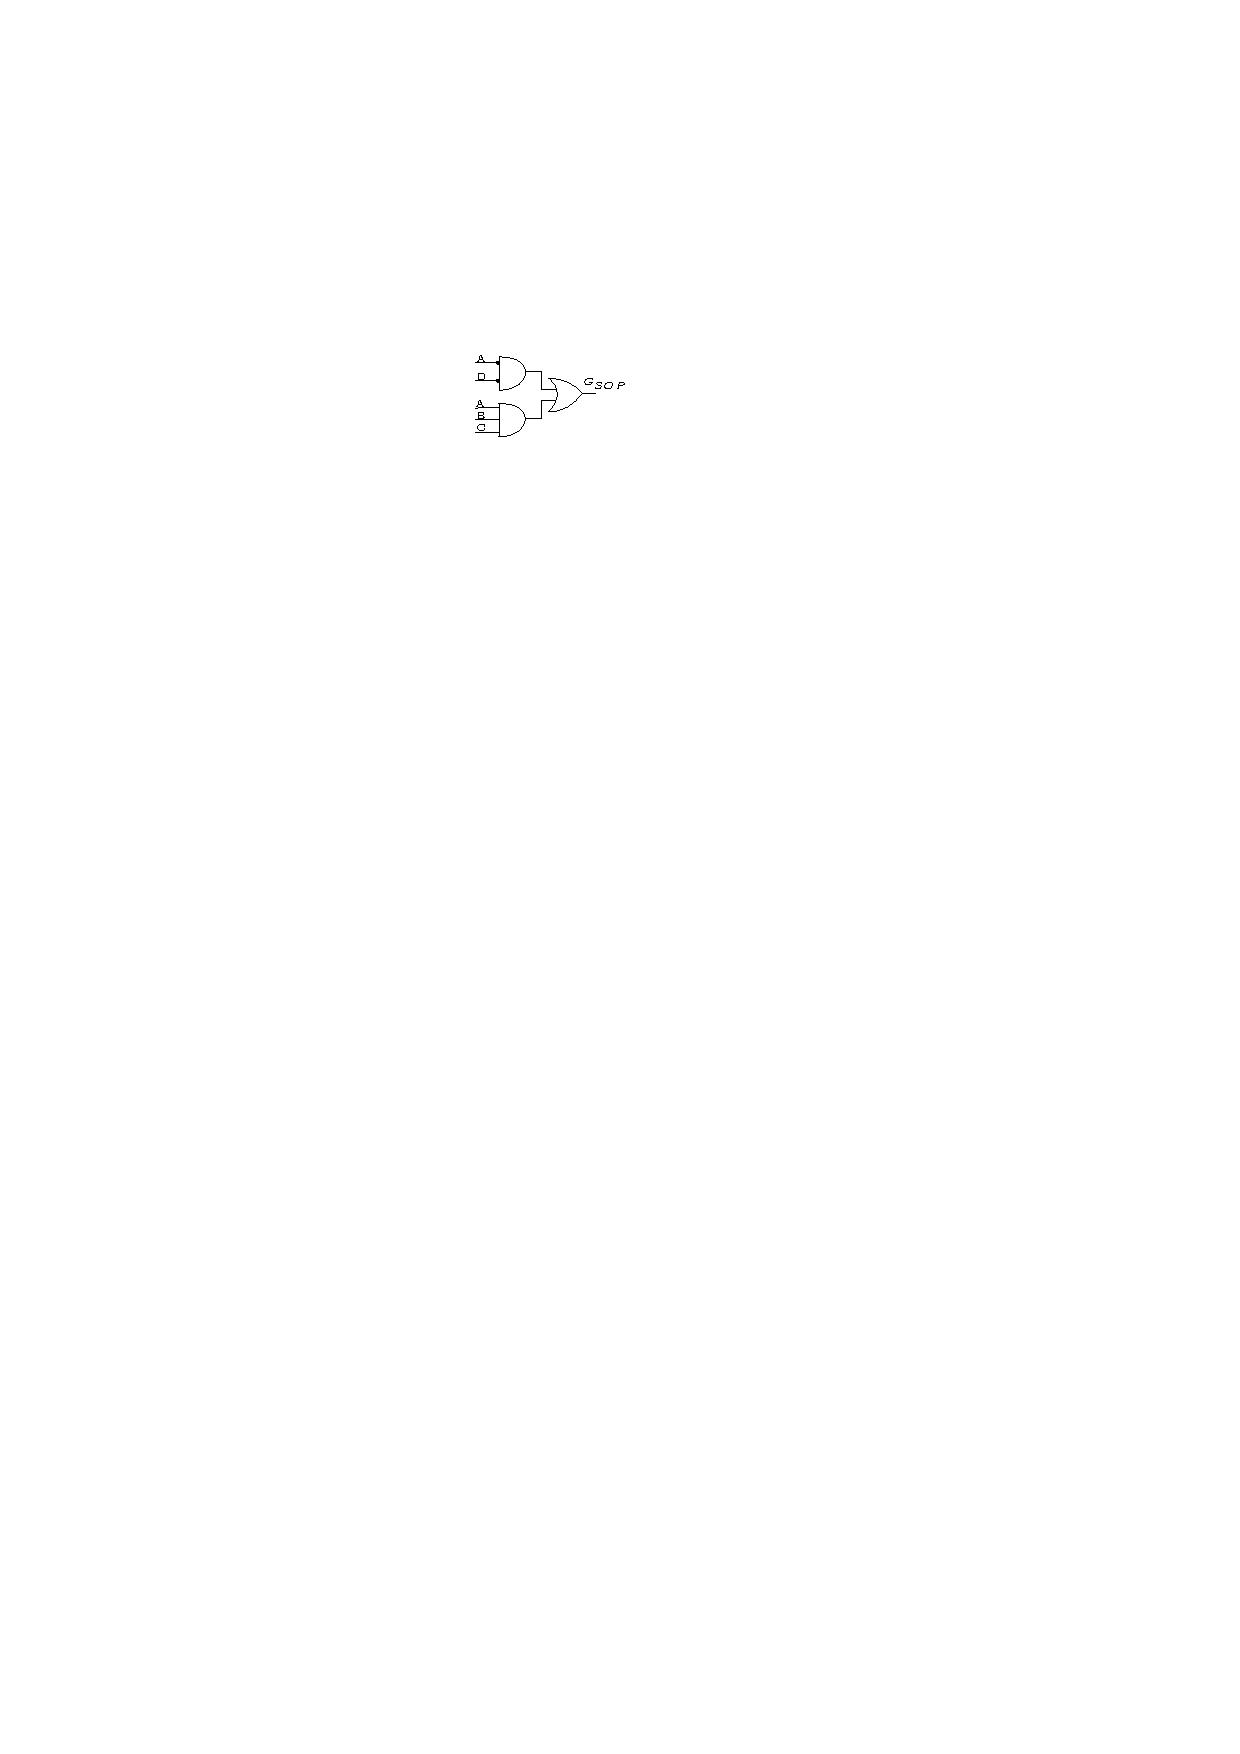
\includegraphics[width=\textwidth]{fig/Q1_G_SOP.pdf}
		\caption{$G_{SOP}$}
		\label{fig:G_SOP}
	\end{subfigure}
	\caption{مدار ساده شده تابع \lr{G}}
	\label{fig:مدار یاده شده جی}
\end{figure}

